\chapter{Elementary Graph Algorithms}

In earlier chapters, we developed data structures to organize collections of independent items: trees, heaps, hash tables, and priority queues. Many problems, though, are about relationships between items. Cities joined by roads. Web pages joined by links. People joined by friendships. Tasks joined by ``must happen before'' arrows. Courses joined by prerequisites. The abstraction that covers all of these is the \emph{graph}. A graph is just a set of dots and a set of lines between dots, yet a wide range of algorithmic problems can be modeled directly as questions on graphs.

This chapter is the foundation for everything graph-related that follows --
minimum spanning trees, shortest paths, network flow. The starting question is how to \emph{store} a graph in a
computer, because that choice affects the cost of everything else. With a graph in
hand, there are two fundamental ways to \emph{explore} it: breadth-first
search, which fans outward in rings, and depth-first search, which plunges
forward and backtracks. Depth-first search also leads to two important tools.
One is \emph{topological sort}, which linearizes a tangle of
dependencies. The other is the discovery of \emph{strongly connected
components}, the tightly knit clusters inside a directed graph. By the end you
will be able to look at almost any ``things and connections'' problem and reach
for the right tool.

\chapterline

\section{What a Graph Is}
\label{ch22:what-is-a-graph}

First the vocabulary. A \emph{graph} $G = (V, E)$ has a set of
\emph{vertices} $V$ (the dots, also called \emph{nodes}) and a set of
\emph{edges} $E$ (the lines). Each edge joins two vertices.

The first distinction: are the edges \emph{directed} or
\emph{undirected}? In an \emph{undirected} graph, an edge $\{u, v\}$ is a
two-way street -- if $u$ is connected to $v$, then $v$ is connected to $u$, with
no preferred direction. Think of friendships, or roads you can drive both ways.
In a \emph{directed} graph (often called a \emph{digraph}), an edge $(u, v)$ is
a one-way arrow from $u$ \emph{to} $v$, and it says nothing about whether you
can get back. Think of one-way streets, web links, or ``task $u$ must finish
before task $v$ starts.''

\begin{intuitionbox}
A useful mental test: if you can imagine standing on a vertex and an edge
``points'' somewhere, it is directed. If the edge is just a wire connecting two
pegs with no arrowhead, it is undirected. Undirected graphs are really a special
case of directed ones where every arrow comes with a matching arrow pointing the
other way. We keep them separate because so many real situations are genuinely
symmetric, and pretending otherwise wastes space.
\end{intuitionbox}

A few more words you will need constantly. Two vertices joined by an edge are
\emph{adjacent} (or \emph{neighbors}). The number of edges touching a vertex is
its \emph{degree}; in a directed graph we split this into \emph{out-degree}
(arrows leaving) and \emph{in-degree} (arrows arriving). A \emph{path} is a
sequence of vertices where each consecutive pair is joined by an edge. A
\emph{cycle} is a path that returns to where it started. A graph with no cycles
is \emph{acyclic}; a directed acyclic graph appears so often it has its own
three-letter name, \emph{DAG}, which we will meet again in topological sort.

\begin{focusbox}
Throughout the chapter we write $V$ for the number of vertices and $E$ for the
number of edges. (Strictly $\abs{V}$ and $\abs{E}$, but everyone abuses notation
and writes $V$ and $E$ inside $O(\cdot)$, and so will we.) Almost every running
time in graph algorithms is some combination of $V$ and $E$, and learning to
read those formulas -- to feel whether $O(V + E)$ is fast and $O(V^2)$ is
wasteful for your particular graph -- is a core skill.
\end{focusbox}

How big can $E$ be relative to $V$? In an undirected graph with no self-loops or
repeated edges, every pair of vertices contributes at most one edge, so
$E \le \binom{V}{2} = \Theta(V^2)$. A graph that has nearly this many edges is
called \emph{dense}; one with only a handful per vertex, so $E = O(V)$, is
\emph{sparse}. Most real graphs -- road networks, social networks, the web --
are very sparse, and this fact drives the main storage decision we are about
to make.

\section{Storing a Graph: Lists versus Matrices}
\label{ch22:representations}

You cannot run an algorithm on a picture. We need to encode those vertices and
edges in memory so an algorithm can traverse them efficiently. There are two
classic encodings, and the trade-off between them matters.

\subsection{The adjacency matrix}

The most literal encoding is a grid. Number the vertices $1, 2, \ldots, V$.
Build a $V \times V$ table $A$ where $A[i][j] = 1$ if there is an edge from $i$
to $j$, and $0$ otherwise. That's the \emph{adjacency matrix}.

\begin{example}
\label{ch22:matrix-example}
Take an undirected graph on four vertices $\{1, 2, 3, 4\}$ with edges
$\{1,2\}$, $\{1,3\}$, $\{2,3\}$, and $\{3,4\}$. Its adjacency matrix is
\[
A =
\begin{array}{c|cccc}
 & 1 & 2 & 3 & 4 \\ \hline
1 & 0 & 1 & 1 & 0 \\
2 & 1 & 0 & 1 & 0 \\
3 & 1 & 1 & 0 & 1 \\
4 & 0 & 0 & 1 & 0
\end{array}
\]
Notice the matrix is \emph{symmetric} across the diagonal: $A[i][j] = A[j][i]$.
That symmetry is exactly what ``undirected'' means in matrix form. For a
directed graph the matrix would generally not be symmetric.
\end{example}

The matrix has two appealing properties. You can answer ``is there an edge
from $i$ to $j$?'' in $O(1)$ time -- one array lookup, no searching. And it
is simple and supports algebraic methods (you will see in a later
chapter that squaring the matrix counts paths of length two). But it has one
serious drawback for large sparse graphs: it always uses $\Theta(V^2)$ space, even if
the graph has only a dozen edges. A social network with a billion users would
need a matrix with $10^{18}$ entries, almost all of them zero, which is
infeasible.

\subsection{The adjacency list}

The adjacency list throws away all those zeros. For each vertex $u$, keep a
little list $\mathit{Adj}[u]$ naming exactly the vertices $u$ connects to.
Nothing more.

\begin{example}
\label{ch22:list-example}
The same graph from Example~\ref{ch22:matrix-example} as adjacency lists:
\[
\begin{aligned}
\mathit{Adj}[1] &= [\,2,\ 3\,] \\
\mathit{Adj}[2] &= [\,1,\ 3\,] \\
\mathit{Adj}[3] &= [\,1,\ 2,\ 4\,] \\
\mathit{Adj}[4] &= [\,3\,]
\end{aligned}
\]
In an undirected graph each edge shows up \emph{twice} -- edge $\{1,2\}$ puts a
$2$ in $\mathit{Adj}[1]$ and a $1$ in $\mathit{Adj}[2]$. So the total length of
all the lists is exactly $2E$. In a directed graph each edge appears once, in
the list of its source vertex, and the total length is $E$. Either way, the
space used is $\Theta(V + E)$: one slot per vertex for the list header, plus one
entry per edge-endpoint.
\end{example}

\begin{center}
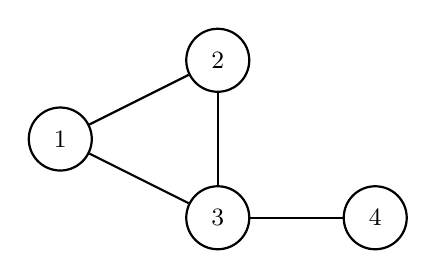
\begin{tikzpicture}[
  vertex/.style={circle,draw,thick,minimum size=8mm,inner sep=0pt},
  every node/.style={font=\small}]
  \node[vertex] (1) at (0,0) {1};
  \node[vertex] (2) at (2,1) {2};
  \node[vertex] (3) at (2,-1) {3};
  \node[vertex] (4) at (4,-1) {4};
  \draw[thick] (1) -- (2);
  \draw[thick] (1) -- (3);
  \draw[thick] (2) -- (3);
  \draw[thick] (3) -- (4);
\end{tikzpicture}
\end{center}

The same four lists, drawn as the linked structure a machine actually holds --
a header array on the left, each pointing to a little chain of its neighbors:

\begin{center}
\begin{tikzpicture}[
  cell/.style={draw,thick,minimum size=7mm,inner sep=2pt,font=\small},
  hdr/.style={cell,fill=sourceblue!12},
  ->,>={Stealth[round]},node distance=8mm]
  \foreach \i/\y in {1/0,2/-0.9,3/-1.8,4/-2.7}{
    \node[hdr] (h\i) at (0,\y) {\i};
  }
  % row 1: 2,3
  \node[cell,right=5mm of h1] (a1) {2}; \node[cell,right=2mm of a1] (a2) {3};
  \draw (h1) -- (a1); \draw (a1) -- (a2);
  % row 2: 1,3
  \node[cell,right=5mm of h2] (b1) {1}; \node[cell,right=2mm of b1] (b2) {3};
  \draw (h2) -- (b1); \draw (b1) -- (b2);
  % row 3: 1,2,4
  \node[cell,right=5mm of h3] (c1) {1}; \node[cell,right=2mm of c1] (c2) {2};
  \node[cell,right=2mm of c2] (c3) {4};
  \draw (h3) -- (c1); \draw (c1) -- (c2); \draw (c2) -- (c3);
  % row 4: 3
  \node[cell,right=5mm of h4] (d1) {3};
  \draw (h4) -- (d1);
\end{tikzpicture}
\end{center}

Now the trade-off is clear. The list uses $\Theta(V + E)$ space, which for a
sparse graph is enormously smaller than $\Theta(V^2)$. The price is that
checking ``is there an edge from $i$ to $j$?'' now means scanning $i$'s list,
which can take up to $O(\deg(i))$ time instead of $O(1)$. For most algorithms --
including every one in this chapter -- you do not ask that question; instead you
ask ``what are all of $u$'s neighbors?'', and the list answers that directly. That is why adjacency lists are the default.

\begin{complexitybox}
For a graph with $V$ vertices and $E$ edges:
\begin{center}
\begin{tabular}{lcc}
\toprule
 & Adjacency list & Adjacency matrix \\
\midrule
Space               & $\Theta(V+E)$ & $\Theta(V^2)$ \\
Edge query $(i,j)$? & $O(\deg i)$   & $O(1)$ \\
List $u$'s neighbors& $\Theta(\deg u)$ & $\Theta(V)$ \\
Best for            & sparse graphs & dense graphs \\
\bottomrule
\end{tabular}
\end{center}
The rule of thumb: \emph{lists for sparse, matrix for dense}. Since real graphs
are usually sparse, lists win in practice almost every time.
\end{complexitybox}

\begin{trapbox}
A classic beginner mistake is to reach for the adjacency matrix because it
``feels simpler,'' then watch the program run out of memory on a graph with a
million vertices. A million-by-million matrix of bytes is a terabyte. The same
graph as lists, if it averages ten edges per vertex, is about ten million
entries -- a few tens of megabytes. Always ask: is my graph sparse? If yes, use
lists.
\end{trapbox}

\section{Breadth-First Search: Exploring in Rings}
\label{ch22:bfs}

Imagine you drop a pebble into a still pond at vertex $s$ (the \emph{source}).
Ripples spread outward in perfect rings: first the vertices one edge away, then
the vertices two edges away, then three, and so on. \emph{Breadth-first search}
(BFS) turns this ripple into an algorithm. It visits vertices in
order of their distance \emph{in number of edges} from $s$, and along the way
it computes the length of the shortest such path to every reachable vertex.

\begin{intuitionbox}
Picture a fire spreading through dry grass from one spot. At minute~1 every cell
touching the start is alight. At minute~2 every cell touching \emph{those}. The
fire never skips ahead -- it cannot reach a cell three steps away before it has
burned through the cells two steps away. BFS is that fire. The ``distance'' it
computes is the minute at which each cell catches.
\end{intuitionbox}

How do we make a computer fan out in rings? We use a \emph{queue} -- a
first-in-first-out line. We process vertices in the exact order we discover
them. Because a vertex at distance $d$ is always discovered before any vertex at
distance $d+1$, and the queue hands them back in arrival order, we are
guaranteed to finish \emph{all} of ring $d$ before touching ring $d+1$.

To keep the bookkeeping straight, we color every vertex one of three colors as
the search runs:
\begin{itemize}
\item \textbf{white} -- not yet discovered (still untouched grass),
\item \textbf{gray} -- discovered but we have not yet looked at all its
neighbors (the burning frontier),
\item \textbf{black} -- discovered and fully explored (burnt out).
\end{itemize}
A vertex goes white $\to$ gray when it first enters the queue, and gray $\to$
black when it leaves the queue after we have scanned its neighbors. We also
record, for each vertex $u$, a distance $d[u]$ (rings from $s$) and a
\emph{predecessor} $\pi[u]$ (the vertex from which we discovered $u$). Those
predecessors, chained together, form the shortest-path tree.

\begin{algorithm}[H]
\caption{BFS$(G, s)$}
\KwIn{Graph $G=(V,E)$ as adjacency lists; source vertex $s$.}
\KwOut{For each $v$: distance $d[v]$ in edges from $s$, and predecessor $\pi[v]$.}
\For{each vertex $u \in V$}{
  $\mathit{color}[u] \gets$ white;\quad $d[u] \gets \infty$;\quad $\pi[u] \gets \textsc{nil}$\;
}
$\mathit{color}[s] \gets$ gray;\quad $d[s] \gets 0$;\quad $\pi[s] \gets \textsc{nil}$\;
$Q \gets$ empty queue;\quad \textsc{Enqueue}$(Q, s)$\;
\While{$Q$ is not empty}{
  $u \gets \textsc{Dequeue}(Q)$\;
  \For{each $v \in \mathit{Adj}[u]$}{
    \If{$\mathit{color}[v] = $ white}{
      $\mathit{color}[v] \gets$ gray\;
      $d[v] \gets d[u] + 1$\;
      $\pi[v] \gets u$\;
      \textsc{Enqueue}$(Q, v)$\;
    }
  }
  $\mathit{color}[u] \gets$ black\;
}
\end{algorithm}

Read it once for the shape. We seed the queue with the source. Then, over and
over, we pull the front vertex $u$, look at each neighbor $v$, and -- only if $v$
is still white (never seen) -- we color it gray, set its distance to one more
than $u$'s, point its predecessor at $u$, and put it in line. Testing for a
white vertex prevents redundant processing: it guarantees that each vertex enters
the queue at most once.

\subsection{A full numeric trace}
\label{ch22:bfs-trace}

Let us run BFS by hand. Here is an undirected graph on six vertices; we will
start from $s = 1$.

\begin{center}
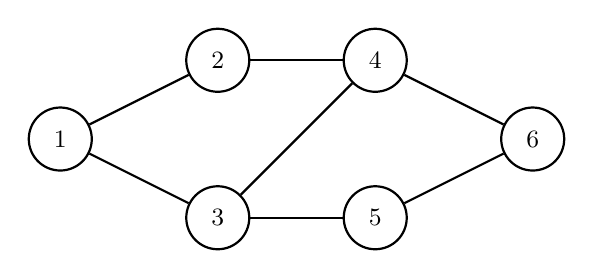
\begin{tikzpicture}[
  vertex/.style={circle,draw,thick,minimum size=8mm,inner sep=0pt},
  every node/.style={font=\small}]
  \node[vertex] (1) at (0,0)   {1};
  \node[vertex] (2) at (2,1)   {2};
  \node[vertex] (3) at (2,-1)  {3};
  \node[vertex] (4) at (4,1)   {4};
  \node[vertex] (5) at (4,-1)  {5};
  \node[vertex] (6) at (6,0)   {6};
  \draw[thick] (1) -- (2);
  \draw[thick] (1) -- (3);
  \draw[thick] (2) -- (4);
  \draw[thick] (3) -- (4);
  \draw[thick] (3) -- (5);
  \draw[thick] (4) -- (6);
  \draw[thick] (5) -- (6);
\end{tikzpicture}
\end{center}

The adjacency lists (with neighbors listed in increasing order) are
$\mathit{Adj}[1]=[2,3]$, $\mathit{Adj}[2]=[1,4]$, $\mathit{Adj}[3]=[1,4,5]$,
$\mathit{Adj}[4]=[2,3,6]$, $\mathit{Adj}[5]=[3,6]$, $\mathit{Adj}[6]=[4,5]$.

We track the queue contents and the distances after each dequeue.

\begin{center}
\begin{tabular}{c l l l}
\toprule
Step & Dequeue & Newly discovered (distance) & Queue after \\
\midrule
0 & --        & $1\,(0)$                 & $[1]$ \\
1 & $1$       & $2\,(1),\ 3\,(1)$        & $[2,3]$ \\
2 & $2$       & $4\,(2)$                 & $[3,4]$ \\
3 & $3$       & $5\,(2)$                 & $[4,5]$ \\
4 & $4$       & $6\,(3)$                 & $[5,6]$ \\
5 & $5$       & (nothing new)            & $[6]$ \\
6 & $6$       & (nothing new)            & $[\,]$ \\
\bottomrule
\end{tabular}
\end{center}

Walk through the interesting moments. At step~2 we dequeue $2$ and look at its
neighbors $1$ and $4$. Vertex $1$ is already black, so we skip it; vertex $4$ is
white, so it becomes gray at distance $d[2]+1 = 2$, with $\pi[4] = 2$. At step~3
we dequeue $3$; among its neighbors $1$ (black) and $4$ (already gray -- we
discovered it a moment ago via $2$) are skipped, but $5$ is white and gets
distance $2$ with $\pi[5]=3$. Notice that $4$ was \emph{not} re-discovered
through $3$: the white check protected it. At step~4 vertex $4$ finally gives us
$6$ at distance $3$. By the time we reach $5$ and $6$, everything is discovered,
so they add nothing.

Final distances from $s=1$:
\[
d[1]=0,\quad d[2]=1,\quad d[3]=1,\quad d[4]=2,\quad d[5]=2,\quad d[6]=3.
\]

It helps to see the same result organized by distance rings (Figure~\ref{ch22:bfs-wavefronts}).
Each band collects vertices at a specific distance from source $s=1$. The bold edges
represent predecessor (tree) edges kept by BFS; notice every bold edge connects a vertex
in ring $d$ to a vertex in ring $d+1$, never skipping across rings.

\begin{figure}[h]
\centering
\begin{tikzpicture}[
  scale=0.92,
  vertex/.style={circle,draw=gray!70,thick,minimum size=8mm,inner sep=0pt,font=\small},
  lbl/.style={font=\scriptsize\scshape, text=gray!80!black}
]
  % Wavefront bands
  \fill[sourceblue!15,rounded corners=4pt] (-0.8,-1.7) rectangle (0.8,1.7);
  \fill[sourceblue!8,rounded corners=4pt] (1.5,-1.7) rectangle (3.3,1.7);
  \fill[sourceblue!4,rounded corners=4pt] (3.9,-1.7) rectangle (5.7,1.7);
  \fill[gray!4,rounded corners=4pt] (6.4,-1.7) rectangle (8.0,1.7);

  \node[vertex,fill=sourceblue!35,draw=sourceblue!80!black] (1) at (0,0)   {1};
  \node[vertex,fill=white] (2) at (2.4,0.85)  {2};
  \node[vertex,fill=white] (3) at (2.4,-0.85) {3};
  \node[vertex,fill=white] (4) at (4.8,0.85)  {4};
  \node[vertex,fill=white] (5) at (4.8,-0.85) {5};
  \node[vertex,fill=white] (6) at (7.2,0)    {6};

  % Tree (predecessor) edges in bold sourceblue
  \draw[very thick,sourceblue,->,>=stealth] (1) -- (2);
  \draw[very thick,sourceblue,->,>=stealth] (1) -- (3);
  \draw[very thick,sourceblue,->,>=stealth] (2) -- (4);
  \draw[very thick,sourceblue,->,>=stealth] (3) -- (5);
  \draw[very thick,sourceblue,->,>=stealth] (4) -- (6);

  % Non-tree edges (discovered already): thin gray dashed
  \draw[thick,gray!60,dashed] (3) -- (4);
  \draw[thick,gray!60,dashed] (5) -- (6);

  % Ring labels
  \node[lbl] at (0,-1.4) {Wave 0: $d=0$};
  \node[lbl] at (2.4,-1.4) {Wave 1: $d=1$};
  \node[lbl] at (4.8,-1.4) {Wave 2: $d=2$};
  \node[lbl] at (7.2,-1.4) {Wave 3: $d=3$};

  % Connecting boundary lines
  \draw[dotted,gray!50] (1.15,-1.7) -- (1.15,1.7);
  \draw[dotted,gray!50] (3.6,-1.7) -- (3.6,1.7);
  \draw[dotted,gray!50] (6.05,-1.7) -- (6.05,1.7);
\end{tikzpicture}
\caption{Breadth-first search as expanding concentric wavefronts. Vertices partition into frontier layers $d = 0, 1, 2, 3$. Bold arrows show the predecessor tree edges discovered during exploration; non-tree edges (dashed) connect vertices either within the same wave or between adjacent waves, confirming that BFS never skips a layer.}
\label{ch22:bfs-wavefronts}
\end{figure}
And the predecessor tree, $\pi[2]=\pi[3]=1$, $\pi[4]=2$, $\pi[5]=3$,
$\pi[6]=4$, encodes one shortest path to each vertex. To recover the path to
$6$, follow predecessors backward: $6 \leftarrow 4 \leftarrow 2 \leftarrow 1$,
i.e.\ $1 \to 2 \to 4 \to 6$, three edges -- exactly $d[6]$.

\begin{labbox}
Re-run the trace, but this time start from $s = 6$ and write out the queue at
every step yourself. Predict the distances before you check them: you should get
$d[6]=0$, the neighbors of $6$ at distance $1$, and so on. Then notice something:
because this graph is undirected, $d_{s=1}[6] = d_{s=6}[1] = 3$. Distance is
symmetric in undirected graphs. Is it symmetric in directed graphs? (No; find a
small directed example that shows why.)
\end{labbox}

\subsection{Why BFS finds shortest paths}
\label{ch22:bfs-correctness}

We claimed BFS computes the shortest distance in edges. Time to make that precise
and prove it. Define $\delta(s, v)$ to be the \emph{true} minimum
number of edges on any path from $s$ to $v$ (and $\infty$ if no path exists).

\begin{formalbox}
\textbf{Theorem (BFS correctness).} After BFS$(G, s)$ terminates, $d[v] =
\delta(s, v)$ for every vertex $v$. The predecessor edges also form a tree in
which the path from $s$ to $v$ is a shortest path.
\end{formalbox}

The argument rests on a loop invariant about the queue: the queue is always a
snapshot of the frontier, and the frontier is never more than one ring deep.

\begin{formalbox}
\textbf{Queue invariant.} At every point during BFS, if the queue holds the
vertices $\langle v_1, v_2, \ldots, v_r \rangle$ from front to back, then
$d[v_r] \le d[v_1] + 1$, and the distances are non-decreasing:
$d[v_1] \le d[v_2] \le \cdots \le d[v_r]$.
\end{formalbox}

Why does this hold? Initially the queue is just $\langle s \rangle$ with
$d[s]=0$, so both conditions hold immediately for the base case. Now suppose they hold and we dequeue the
front $v_1$. Whatever new vertices we enqueue get distance $d[v_1]+1$, and they
go to the \emph{back}. Check both parts. Sortedness: the old back had
$d[v_r] \le d[v_1]+1$, so appending vertices with distance $d[v_1]+1$ keeps the
queue non-decreasing. Two-ring span: the new front is $v_2$ with
$d[v_2] \ge d[v_1]$, and the new back has distance at most
$d[v_1]+1 \le d[v_2]+1$. (If the queue empties and refills, the same check
applies with $v_1$ alone.) So the queue stays sorted by distance and spans at
most two adjacent rings.

From this invariant the theorem follows by induction on distance. Every vertex
$v$ first becomes gray when some neighbor $u$ with $d[u] = \delta(s,v) - 1$
dequeues; at that instant $d[v]$ is set to $d[u]+1 = \delta(s,v)$, and it is
never changed again. Why can't a farther vertex $w$ (with $d[w] \ge \delta(s,v)$)
discover $v$ first? Because the queue is sorted, every vertex at distance
$\delta(s,v)-1$ is dequeued before any vertex at distance $\delta(s,v)$ or more,
so $v$'s correct-ring neighbor always gets there first. And $d[v]$ can never be
\emph{smaller} than $\delta(s,v)$, because every value BFS assigns is the length
of an actual path from $s$. CLRS Section~20.2 gives the full proof; the picture
to keep is the ordered queue.

\begin{walkbox}
Go for a walk and convince yourself, without any algebra, why a queue and not a
stack is what makes BFS find shortest paths. What goes wrong if you swap the
queue for a stack -- if you always explore the \emph{most recently} discovered
vertex instead of the oldest? (Hint: you get a different, equally famous
algorithm, and it does \emph{not} respect rings. That is the next section.)
\end{walkbox}

\subsection{The running time of BFS}
\label{ch22:bfs-time}

Rather than quote the cost, let us derive it. Two things happen during BFS:
queue operations, and scanning adjacency lists.

\emph{Queue operations.} Each vertex is colored gray exactly once -- the moment
it is enqueued -- and the white check forbids enqueuing it again. So each vertex
is enqueued once and dequeued once: $O(V)$ total queue operations, each $O(1)$.

\emph{Scanning lists.} When a vertex $u$ is dequeued, we scan its entire
adjacency list $\mathit{Adj}[u]$ once, doing $O(1)$ work per neighbor. Since each
vertex is dequeued once, each adjacency list is scanned once. The total length of
all adjacency lists is $\Theta(E)$ (counting each edge once if directed, twice if
undirected). So all the scanning costs $\Theta(E)$.

Adding the one-time initialization of $\Theta(V)$, we get:

\begin{complexitybox}
\textbf{BFS runs in $O(V + E)$ time} and uses $O(V)$ extra space for the queue,
colors, distances, and predecessors. This is \emph{linear in the size of the
graph} -- you cannot do better, because you must at least look at every vertex
and edge. The $+$ matters: you pay for vertices \emph{and} edges separately,
never their product. This is the payoff of adjacency lists; the same algorithm on an
adjacency matrix would cost $O(V^2)$, because scanning a vertex's neighbors means
walking a whole matrix row of length $V$.
\end{complexitybox}

\section{Depth-First Search: Plunge and Backtrack}
\label{ch22:dfs}

Breadth-first search is cautious: it never steps into ring $d+1$ until ring $d$
is fully mapped. \emph{Depth-first search} (DFS) does the opposite: from
wherever it stands, it follows the first unexplored edge it sees, then down the first edge from \emph{there}, plunging
ever deeper until it hits a dead end -- a vertex whose neighbors are all already
visited. Only then does it \emph{backtrack} one step and try the next edge.

\begin{intuitionbox}
DFS is how you explore a maze with a ball of string and a piece of chalk. You
walk forward, chalking each junction so you know you have been there, always
taking some unmarked corridor. When every corridor from your current spot is
already chalked, you reel in the string one junction and try another corridor
there. You only stop when the string is fully reeled in and you are back at the
start with no fresh corridors anywhere. The string is the recursion stack; the
chalk is the color.
\end{intuitionbox}

Because DFS backtracks, it is naturally \emph{recursive}: ``explore $u$'' means
``for each neighbor, if it is white, explore it.'' The recursion stack remembers
the trail of string for us. We keep the same white/gray/black coloring as BFS,
but now we also stamp each vertex with two \emph{timestamps} from a global clock
that ticks once per event:
\begin{itemize}
\item $d[u]$, the \emph{discovery time}, when $u$ turns gray (we first arrive),
\item $f[u]$, the \emph{finish time}, when $u$ turns black (we leave for good,
having explored everything reachable below it).
\end{itemize}
These timestamps record the nested structure of the search, and they are what
make topological sort and strongly connected
components possible. Every vertex gets a discovery and a finish time, so the
clock runs from $1$ to $2V$.

Unlike BFS, DFS does not need a source: it sweeps over \emph{all} vertices,
launching a fresh exploration from each white one, so that even a disconnected
graph is fully covered. The result is a \emph{forest} of trees, one per launch.

\begin{algorithm}[H]
\caption{DFS$(G)$}
\KwIn{Graph $G=(V,E)$ as adjacency lists.}
\KwOut{Discovery/finish times $d[u], f[u]$ and predecessors $\pi[u]$.}
\For{each vertex $u \in V$}{
  $\mathit{color}[u] \gets$ white;\quad $\pi[u] \gets \textsc{nil}$\;
}
$\mathit{time} \gets 0$\;
\For{each vertex $u \in V$}{
  \If{$\mathit{color}[u] = $ white}{
    \textsc{DFS-Visit}$(G, u)$\;
  }
}
\end{algorithm}

\begin{algorithm}[H]
\caption{DFS-Visit$(G, u)$}
$\mathit{time} \gets \mathit{time} + 1$;\quad $d[u] \gets \mathit{time}$\;
$\mathit{color}[u] \gets$ gray\;
\For{each $v \in \mathit{Adj}[u]$}{
  \If{$\mathit{color}[v] = $ white}{
    $\pi[v] \gets u$\;
    \textsc{DFS-Visit}$(G, v)$\;
  }
}
$\mathit{color}[u] \gets$ black\;
$\mathit{time} \gets \mathit{time} + 1$;\quad $f[u] \gets \mathit{time}$\;
\end{algorithm}

\subsection{A full numeric trace}
\label{ch22:dfs-trace}

Let us run DFS on a \emph{directed} graph -- the timestamps are most interesting
there. Consider six vertices with arrows:
\[
1 \to 2,\quad 1 \to 4,\quad 2 \to 3,\quad 3 \to 1,\quad 4 \to 3,\quad 5 \to 4,
\quad 5 \to 6,\quad 6 \to 6.
\]

\begin{center}
\begin{tikzpicture}[
  vertex/.style={circle,draw,thick,minimum size=8mm,inner sep=0pt},
  every node/.style={font=\small},
  ->,>={Stealth[round]}]
  \node[vertex] (1) at (0,0)   {1};
  \node[vertex] (2) at (2,0.8) {2};
  \node[vertex] (3) at (2,-0.8){3};
  \node[vertex] (4) at (4,0.8) {4};
  \node[vertex] (5) at (4,-0.8){5};
  \node[vertex] (6) at (6,-0.8){6};
  \draw[thick] (1) -- (2);
  \draw[thick] (1) to [out=60, in=130] (4);
  \draw[thick] (2) -- (3);
  \draw[thick] (3) -- (1);
  \draw[thick] (4) -- (3);
  \draw[thick] (5) -- (4);
  \draw[thick] (5) -- (6);
  \draw[thick] (6) to [out=30,in=-30,looseness=8] (6);
\end{tikzpicture}
\end{center}

We process vertices in numeric order and, within each list, neighbors in
increasing order. The clock starts at $0$.

We launch from $1$ (time becomes $1$, $d[1]=1$). Its first white neighbor is
$2$ ($d[2]=2$). From $2$ we go to $3$ ($d[3]=3$). From $3$ the only neighbor is
$1$, which is \emph{gray} (still on the stack) -- skip it. So $3$ has no white
neighbor; it finishes: $f[3]=4$. Back at $2$: no more neighbors, finish
$f[2]=5$. Back at $1$: next neighbor $4$ is white ($d[4]=6$). From $4$ the
neighbor $3$ is now \emph{black} -- skip. So $4$ finishes $f[4]=7$. Back at $1$:
no more neighbors, finish $f[1]=8$.

The outer loop now looks for the next white vertex. Vertices $2,3,4$ are black;
$5$ is white. Launch from $5$ ($d[5]=9$). Neighbor $4$ is black -- skip.
Neighbor $6$ is white ($d[6]=10$). From $6$, the only neighbor is $6$ itself,
which is gray -- skip. Finish $f[6]=11$. Back at $5$: done, $f[5]=12$.

Collecting the stamps as $(d, f)$ pairs:
\begin{center}
\begin{tabular}{ccccccc}
\toprule
Vertex & 1 & 2 & 3 & 4 & 5 & 6 \\
\midrule
$d$ & 1 & 2 & 3 & 6 & 9 & 10 \\
$f$ & 8 & 5 & 4 & 7 & 12& 11 \\
\bottomrule
\end{tabular}
\end{center}

The DFS forest has two trees: one rooted at $1$ (containing $1,2,3,4$) and one
rooted at $5$ (containing $5,6$). It is worth redrawing the graph as that
forest, with each non-tree edge labeled by its kind (we classify the edges in
the next subsection); the solid edges are the tree, and the dashed ones are the
back and cross edges that DFS \emph{walked but did not build the tree from}.

\begin{center}
\begin{tikzpicture}[
  vertex/.style={circle,draw,thick,minimum size=9mm,inner sep=0pt,font=\small},
  ->,>={Stealth[round]}]
  % tree 1
  \node[vertex] (1) at (0,0)    {1};
  \node[vertex] (2) at (0,-1.6) {2};
  \node[vertex] (3) at (0,-3.2) {3};
  \node[vertex] (4) at (2,-1.6) {4};
  % tree 2
  \node[vertex] (5) at (5,0)    {5};
  \node[vertex] (6) at (5,-1.6) {6};
  % tree edges (solid)
  \draw[very thick,sourceblue] (1) -- (2);
  \draw[very thick,sourceblue] (2) -- (3);
  \draw[very thick,sourceblue] (1) -- (4);
  \draw[very thick,sourceblue] (5) -- (6);
  % back edges (dashed red)
  \draw[dashed,thick,trapred] (3) to[out=120,in=-120,looseness=1.3] node[left,font=\scriptsize]{back} (1);
  \draw[dashed,thick,trapred] (6) to[out=-30,in=30,looseness=8] node[right,font=\scriptsize]{back} (6);
  % cross edges (dashed purple)
  \draw[dashed,thick,structurepurple] (4) -- node[right,font=\scriptsize,pos=0.55]{cross} (3);
  \draw[dashed,thick,structurepurple] (5) to[out=180,in=70] node[above,font=\scriptsize,pos=0.3]{cross} (4);
\end{tikzpicture}
\end{center}

\subsection{The parenthesis structure}
\label{ch22:parenthesis}

Treat the intervals $[d[u], f[u]]$ as if each vertex opens a parenthesis at
$d[u]$ and closes it at $f[u]$. Writing them out in time order gives a nested
string:
\[
\underbrace{(_1\ \underbrace{(_2\ \underbrace{(_3\ )_3}_{[3,4]}\ )_2}_{[2,5]}\ \underbrace{(_4\ )_4}_{[6,7]}\ )_1}_{[1,8]}\quad
\underbrace{(_5\ \underbrace{(_6\ )_6}_{[10,11]}\ )_5}_{[9,12]}
\]
They never \emph{cross}. Vertex $3$'s interval $[3,4]$ sits entirely inside
$2$'s $[2,5]$, which sits inside $1$'s $[1,8]$. This nesting holds in every
DFS run, and it is the most useful structural property of depth-first
search. Figure~\ref{ch22:dfs-parenthesis}
plots these intervals against the clock.

\begin{figure}[h]
\centering
\begin{tikzpicture}[
  scale=0.92,
  every node/.style={font=\footnotesize},
  ruler/.style={font=\tiny, text=gray!80!black},
  lbl/.style={font=\scriptsize\scshape, text=gray!80!black},
  intbox/.style={draw=gray!70, rounded corners=2pt, thick}
]
  % Time ruler at the top
  \node[lbl, anchor=west] at (-2.0, 4.2) {DFS Discovery/Finish Timeline ($t=1\dots 12$)};
  \draw[thick, gray!60] (0, 3.6) -- (11, 3.6);
  \foreach \t in {1,2,...,12} {
    \pgfmathsetmacro{\x}{(\t-1)*1.0}
    \draw[gray!60] (\x, 3.6) -- (\x, 3.75);
    \node[ruler] at (\x, 3.95) {\t};
    \draw[dotted, gray!25] (\x, -0.3) -- (\x, 3.55);
  }

  % Row labels (left column)
  \node[font=\footnotesize\bfseries, anchor=east] at (-0.3, 3.0) {Vertex $1$};
  \node[font=\footnotesize\bfseries, anchor=east] at (-0.3, 2.4) {Vertex $2$};
  \node[font=\footnotesize\bfseries, anchor=east] at (-0.3, 1.8) {Vertex $3$};
  \node[font=\footnotesize\bfseries, anchor=east] at (-0.3, 1.2) {Vertex $4$};
  \node[font=\footnotesize\bfseries, anchor=east] at (-0.3, 0.6) {Vertex $5$};
  \node[font=\footnotesize\bfseries, anchor=east] at (-0.3, 0.0) {Vertex $6$};

  % Intervals [d, f] with width (f-d)*1.0, positioned at x = d-1
  % Vertex 1: [1, 8] -> x from 0 to 7
  \draw[intbox, fill=sourceblue!20, draw=sourceblue!80!black] (0, 2.8) rectangle (7, 3.2);
  \node[font=\scriptsize\bfseries, text=sourceblue!90!black] at (3.5, 3.0) {$[1, 8]$};

  % Vertex 2: [2, 5] -> x from 1 to 4
  \draw[intbox, fill=targetgreen!22, draw=targetgreen!80!black] (1, 2.2) rectangle (4, 2.6);
  \node[font=\scriptsize\bfseries, text=targetgreen!90!black] at (2.5, 2.4) {$[2, 5]$};

  % Vertex 3: [3, 4] -> x from 2 to 3
  \draw[intbox, fill=quotientorange!28, draw=quotientorange!90!black] (2, 1.6) rectangle (3, 2.0);
  \node[font=\scriptsize\bfseries, text=quotientorange!95!black] at (2.5, 1.8) {$[3, 4]$};

  % Vertex 4: [6, 7] -> x from 5 to 6
  \draw[intbox, fill=targetgreen!22, draw=targetgreen!80!black] (5, 1.0) rectangle (6, 1.4);
  \node[font=\scriptsize\bfseries, text=targetgreen!90!black] at (5.5, 1.2) {$[6, 7]$};

  % Vertex 5: [9, 12] -> x from 8 to 11
  \draw[intbox, fill=sourceblue!20, draw=sourceblue!80!black] (8, 0.4) rectangle (11, 0.8);
  \node[font=\scriptsize\bfseries, text=sourceblue!90!black] at (9.5, 0.6) {$[9, 12]$};

  % Vertex 6: [10, 11] -> x from 9 to 10
  \draw[intbox, fill=targetgreen!22, draw=targetgreen!80!black] (9, -0.2) rectangle (10, 0.2);
  \node[font=\scriptsize\bfseries, text=targetgreen!90!black] at (9.5, 0.0) {$[10, 11]$};

  % Annotations on nesting
  \node[font=\tiny\itshape, text=gray!70!black, anchor=west] at (3.2, 1.8) {$[3,4] \subset [2,5] \subset [1,8]$};
  \node[font=\tiny\itshape, text=gray!70!black, anchor=west] at (6.2, 1.2) {$[6,7] \subset [1,8]$};
  \node[font=\tiny\itshape, text=gray!70!black, anchor=west] at (7.2, 3.0) {Tree 1};
  \node[font=\tiny\itshape, text=gray!70!black, anchor=west] at (11.1, 0.6) {Tree 2};
\end{tikzpicture}
\caption{The Parenthesis Theorem visualized as interval nesting across the discrete DFS clock. Each interval $[d[u], f[u]]$ represents the active lifetime of vertex $u$ on the recursive call stack. Descendant intervals ($[3,4]$ inside $[2,5]$ inside $[1,8]$) nest strictly within their ancestors. Disjoint intervals ($[1,8]$ and $[9,12]$) correspond to separate trees in the DFS forest. No two intervals ever partially overlap without containment.}
\label{ch22:dfs-parenthesis}
\end{figure}

\begin{formalbox}
\textbf{Parenthesis theorem.} In any DFS, for any two vertices $u$ and $v$,
exactly one of these holds:
\begin{itemize}
\item the intervals $[d[u],f[u]]$ and $[d[v],f[v]]$ are completely
\textbf{disjoint}, and neither is a descendant of the other in the forest;
\item one interval is entirely \textbf{contained} in the other, and the inner
vertex is a descendant of the outer in the DFS forest.
\end{itemize}
The forbidden case -- intervals that overlap but neither contains the other --
\textbf{never happens.}
\end{formalbox}

Why must this be true? Because the recursion stack enforces nesting. If $u$ is
discovered while $v$ is still gray (on the stack), then $u$ is being explored
\emph{inside} $v$'s call, so $u$ must finish before control returns to $v$ --
forcing $[d[u],f[u]]$ inside $[d[v],f[v]]$. If instead $u$ is discovered after
$v$ has already finished, the two calls never overlap in time at all. There is no
third option: a vertex is either still on the stack or already off it.

\begin{focusbox}
The slogan: \emph{descendant intervals nest inside ancestor intervals; unrelated
intervals are disjoint}. Equivalently, $v$ is a descendant of $u$ in the DFS
forest \emph{if and only if} $d[u] < d[v] < f[v] < f[u]$. Most DFS
applications -- topological sort, strongly connected components, finding
articulation points -- rely on this nesting fact.
\end{focusbox}

\subsection{Classifying the edges}
\label{ch22:edge-classification}

This nesting structure lets us classify every edge of $G$ during the search. As
DFS walks an edge $(u, v)$ -- meaning we are at gray vertex $u$ and looking at
neighbor $v$ -- the \emph{color of $v$} tells us exactly what kind of edge it
is. There are four kinds:

\begin{itemize}
\item \textbf{Tree edge}: $v$ is white. We are discovering $v$ for the first
time through this edge. Tree edges are the solid edges of the DFS forest.
\item \textbf{Back edge}: $v$ is gray. Then $v$ is still on the stack -- it is an
\emph{ancestor} of $u$. The edge points backward, up toward the root. Back edges
are the exact witnesses to cycles.
\item \textbf{Forward edge}: $v$ is black and $d[u] < d[v]$. Then $v$ is a
\emph{descendant} of $u$ that we already finished exploring by another route. The
edge skips forward to an already-explored descendant.
\item \textbf{Cross edge}: $v$ is black and $d[u] > d[v]$. Then $v$ is in a
different subtree (or an earlier-finished sibling). The edge crosses between
branches.
\end{itemize}

\begin{intuitionbox}
The color of the vertex you are looking at almost \emph{determines} the edge type:
white means tree, gray means back, black means forward-or-cross, and you split
the last case by comparing discovery times. You never have to do anything extra
to classify edges; the coloring the search already maintains gives the
answer.
\end{intuitionbox}

Figure~\ref{ch22:fig-edge-types} illustrates the geometric meaning of each classification relative to the DFS tree.

\begin{figure}[htbp]
\centering
\begin{tikzpicture}[
  scale=0.95,
  vertex/.style={circle, draw=gray!70, fill=gray!5, thick, minimum size=8.5mm, inner sep=0pt, font=\small},
  tree edge/.style={->, >=stealth, very thick, sourceblue},
  back edge/.style={->, >=stealth, thick, dashed, trapred},
  fwd edge/.style={->, >=stealth, thick, dashed, targetgreen},
  cross edge/.style={->, >=stealth, thick, dashed, structurepurple},
  lbl/.style={font=\scriptsize, align=center, inner sep=2pt}
]
  % Background indicators FIRST
  \draw[gray!30, dotted, thick, rounded corners=4pt, fill=sourceblue!2] (-3.8, -0.4) rectangle (-1.0, 1.3);
  \node[font=\tiny, text=gray!55] at (-2.4, -0.2) {Branch 1 (finished)};

  \draw[gray!30, dotted, thick, rounded corners=4pt, fill=gray!3] (0.8, -2.2) rectangle (3.4, 1.3);
  \node[font=\tiny, text=gray!55] at (2.1, -2.0) {Branch 2 (active)};

  % Nodes
  \node[vertex] (u) at (0, 2.2)    {$u$};
  \node[vertex] (v) at (-2.4, 0.5) {$v$};
  \node[vertex] (x) at (2.0, 0.5)  {$x$};
  \node[vertex] (z) at (2.0, -1.3) {$z$};

  % Tree edges (solid blue)
  \draw[tree edge] (u) -- node[lbl, above left=2pt, text=sourceblue!90!black] {Tree} (v);
  \draw[tree edge] (u) -- node[lbl, above right=2pt, text=sourceblue!90!black] {Tree} (x);
  \draw[tree edge] (x) -- node[lbl, right=2pt, text=sourceblue!90!black] {Tree} (z);

  % Back edge: from v back up to ancestor u
  \draw[back edge] (v) to [out=110, in=190] 
    node[lbl, left=2pt, text=trapred] {\textbf{Back edge}\\($u$ gray)} (u);

  % Forward edge: from u down to descendant z
  \draw[fwd edge] (u) to [out=-15, in=35, looseness=1.3] 
    node[lbl, right=2pt, text=targetgreen!80!black] {\textbf{Forward edge}\\($z$ black, $d[u] < d[z]$)} (z);

  % Cross edge: from x across to already-finished v
  \draw[cross edge] (x) -- 
    node[lbl, below=4pt, text=structurepurple] {\textbf{Cross edge}\\[-1pt]{\tiny($v$ finished black)}} (v);
\end{tikzpicture}
\caption{Classification of edges during Depth-First Search. Solid blue lines are tree edges forming the DFS forest. Non-tree edges: \emph{back edges} return up to a gray ancestor on the active call stack (detecting a cycle); \emph{forward edges} skip down to an already-finished descendant; and \emph{cross edges} connect across to an already-finished vertex in an earlier-explored branch.}
\label{ch22:fig-edge-types}
\end{figure}

In our trace above, walk the edges: $1\to2$, $2\to3$, $1\to4$ are tree edges
(each found a white vertex). $3\to1$ is a \emph{back edge} -- when we looked at
$1$ from $3$, vertex $1$ was gray (an ancestor). $4\to3$ is a \emph{cross edge}
-- when we looked at $3$ from $4$, vertex $3$ was already black and $d[4]=6 >
d[3]=3$. The self-loop $6\to6$ is a back edge (a vertex is its own ancestor in
the degenerate sense). The edge $5\to4$ is also a cross edge: $4$ was black with
$d[4]=6 < d[5]=9$.

\begin{formalbox}
\textbf{Cycle test.} A directed graph has a cycle \emph{if and only if} some DFS
of it produces a back edge.
\end{formalbox}

This is the key to detecting cycles, and it has a one-line proof both ways. If
there is a back edge $(u, v)$, then $v$ is an ancestor of $u$, so the tree path
from $v$ down to $u$ plus the edge $(u, v)$ is a cycle. Conversely, if there is a
cycle, consider the first vertex $v$ on it that DFS discovers. At that moment
every other vertex of the cycle is still white, so the rest of the cycle is a
white path out of $v$. DFS cannot finish $v$ while a white path still leads out
of it, so all of those vertices become descendants of $v$. In particular the cycle's last vertex $u$, whose edge
$(u, v)$ returns to $v$, is a descendant of $v$, and when DFS examines $(u,v)$ the
vertex $v$ is still gray: that is a back edge. We will lean on exactly this fact
in topological sort.

\begin{trapbox}
Edge classification depends on the \emph{order} in which DFS happens to visit
vertices and neighbors. The same graph, explored in a different order, can label
the same edge differently (a forward edge in one run might not appear as such in
another). But two things never change: tree and back edges in an \emph{undirected}
graph are the only two kinds that can appear, and a back edge appears if and only
if the graph has a cycle. Do not over-read a specific classification as a property
of the graph; read it as a property of \emph{this} traversal.
\end{trapbox}

\subsection{The running time of DFS}

The accounting is the same shape as BFS. The initialization loop is $\Theta(V)$.
\textsc{DFS-Visit} is called exactly once per vertex (the white check guards it),
contributing $\Theta(V)$ across all calls. Inside those calls, we scan each
adjacency list exactly once, and the lists total $\Theta(E)$ in length.

\begin{complexitybox}
\textbf{DFS runs in $\Theta(V + E)$ time}, linear in the graph, using $O(V)$
space for colors, timestamps, predecessors, and the recursion stack (whose depth
is at most $V$). Like BFS, it touches every vertex and edge a constant number of
times and never their product. If your DFS ever seems to cost more, you are
probably re-scanning lists or testing edges through a matrix -- check that.
\end{complexitybox}

\section{Topological Sort: Untangling Dependencies}
\label{ch22:toposort}

Now an application. Suppose you must do a list of tasks, and some tasks
depend on others: you cannot put your socks on after your shoes, cannot compile
a file before its headers, cannot take Algorithms before Discrete Math. Model
each task as a vertex and draw an arrow $u \to v$ meaning ``$u$ must come before
$v$.'' The dependencies form a \emph{directed graph}, and if your requirements
are sane -- no task transitively requires itself -- that graph is a \emph{DAG}, a
directed acyclic graph.

The question: \emph{can you line all the tasks up in a single row so that every
arrow points forward}? Such a linear order is a \emph{topological sort}. It tells
you a valid sequence in which to actually do everything.

\begin{intuitionbox}
Think of the famous ``getting dressed'' graph: underwear before pants, pants
before belt, socks before shoes, shirt before tie, tie before jacket. There is
no single ``correct'' order -- you might do socks-then-underwear or
underwear-then-socks, it doesn't matter -- but \emph{any} order you pick must
respect every arrow. A topological sort produces one such legal dressing
sequence. There can be many; you just need one.
\end{intuitionbox}

DFS already computes this at almost no extra cost. Recall the finish times
$f[u]$. The method is:

\begin{formalbox}
\textbf{Topological sort via DFS.} Run DFS on the DAG. As each vertex finishes
(turns black), prepend it to the front of a list. When DFS ends, the list is a
valid topological order. Equivalently: output the vertices in \emph{decreasing
order of finish time} $f[u]$.
\end{formalbox}

\begin{algorithm}[H]
\caption{Topological-Sort$(G)$}
\KwIn{A directed acyclic graph $G=(V,E)$.}
\KwOut{A list of vertices in topological order.}
Call DFS$(G)$, computing finish times $f[u]$ for all $u$\;
\emph{(as each vertex finishes, push it onto the front of a linked list $L$)}\;
\Return{$L$}\;
\end{algorithm}

Why does ordering by finish time work? The proof rests on one claim:

\begin{formalbox}
\textbf{Claim.} If $G$ is a DAG and DFS is run on it, then for every edge
$(u, v)$ we have $f[u] > f[v]$.
\end{formalbox}

The argument is short. Consider any edge $(u, v)$. When DFS
explores $u$ and looks at $v$, $v$ has some color.
\begin{itemize}
\item $v$ cannot be \emph{gray}. If it were, $(u,v)$ would be a back edge, and a
back edge means a cycle -- but $G$ is acyclic. Contradiction. (This is the only
place we use the no-cycles assumption, and it is essential.)
\item If $v$ is \emph{white}, then $v$ becomes a descendant of $u$, so by the
parenthesis theorem $v$ finishes before $u$: $f[v] < f[u]$. Good.
\item If $v$ is \emph{black}, then $v$ already finished while $u$ is still gray,
so $f[v] < d[u] < f[u]$. Good.
\end{itemize}
In every possible case, $f[v] < f[u]$. So listing vertices by decreasing finish
time puts $u$ before $v$ for \emph{every} edge $(u,v)$ -- which is exactly the
definition of a topological order. Done.

\subsection{A worked topological sort}

Take this small DAG of morning tasks:
\[
\text{wake} \to \text{shower},\quad
\text{shower} \to \text{dress},\quad
\text{wake} \to \text{coffee},\quad
\text{dress} \to \text{leave},\quad
\text{coffee} \to \text{leave}.
\]
Label them $w, s, d, c, \ell$. Run DFS starting at $w$, neighbors in the order
listed. We discover $w$ ($d[w]=1$), then $s$ ($d=2$), then $d$ ($d=3$), then
$\ell$ ($d=4$). From $\ell$ there are no out-edges, so $\ell$ finishes
$f[\ell]=5$. Back up: $d$ finishes $f[d]=6$, $s$ finishes $f[s]=7$. Back at $w$,
next neighbor $c$ is white: discover $c$ ($d=8$); its neighbor $\ell$ is black,
skip; $c$ finishes $f[c]=9$; finally $w$ finishes $f[w]=10$.

Finish times: $f[w]=10$, $f[c]=9$, $f[s]=7$, $f[d]=6$, $f[\ell]=5$. Sorting by
\emph{decreasing} finish time:
\[
w\ (10),\quad c\ (9),\quad s\ (7),\quad d\ (6),\quad \ell\ (5).
\]
So a valid order is: \textbf{wake, coffee, shower, dress, leave}. Drawn on a
line, with every vertex placed left-to-right by decreasing finish time, the
point of the claim becomes visible: \emph{every} edge points rightward.

\begin{center}
\begin{tikzpicture}[
  vertex/.style={circle,draw,thick,minimum size=8mm,inner sep=0pt,font=\small},
  ->,>={Stealth[round]}]
  \node[vertex] (w) at (0,0)  {$w$};
  \node[vertex] (c) at (2,0)  {$c$};
  \node[vertex] (s) at (4,0)  {$s$};
  \node[vertex] (d) at (6,0)  {$d$};
  \node[vertex] (l) at (8,0)  {$\ell$};
  \foreach \v/\t in {w/10,c/9,s/7,d/6,l/5}{
    \node[font=\scriptsize,gray] at ($(\v)+(0,-0.85)$) {$f=\t$};
  }
  \draw[thick,sourceblue] (w) to[out=45,in=135] (s);
  \draw[thick,sourceblue] (w) to[out=30,in=150] (c);
  \draw[thick,sourceblue] (s) to[out=-35,in=-145] (d);
  \draw[thick,sourceblue] (d) -- (l);
  \draw[thick,sourceblue] (c) to[out=-45,in=-135] (l);
\end{tikzpicture}
\end{center}

Check every
edge: $w$ before $s$ and $c$ (yes), $s$ before $d$ (yes), $d$ before $\ell$
(yes), $c$ before $\ell$ (yes). Every arrow points forward in the list. Note
this is not the \emph{only} valid order -- ``wake, shower, dress, coffee,
leave'' also works -- but DFS handed us one legal answer with no extra effort.

\begin{aestheticbox}
Topological sort appears in many systems. \texttt{make} and every modern
build system topologically sorts your source files so headers compile before the
code that includes them. Spreadsheet engines topologically sort cell formulas so
a cell is computed after the cells it references. Package managers
(\texttt{apt}, \texttt{npm}, \texttt{pip}) topologically sort dependencies to
decide install order. Course-planning tools sort prerequisites. Every time a
program must do things ``in a valid order given constraints,'' it is usually
doing a topological sort. And because it is just one DFS, it costs only $O(V+E)$.
\end{aestheticbox}

\begin{walkbox}
On your walk, ponder: what happens if you run Topological-Sort on a directed
graph that actually contains a cycle? Trace what the DFS does -- it produces a
back edge. Could you modify Topological-Sort to \emph{detect} the cycle and report ``these tasks
have a circular dependency'' instead of silently producing garbage? (You can: it
is exactly the back-edge test from the previous section.)
\end{walkbox}

\section{Strongly Connected Components}
\label{ch22:scc}

Our last application. In a \emph{directed} graph, two vertices $u$
and $v$ are \emph{strongly connected} if you can get from $u$ to $v$ \emph{and}
from $v$ back to $u$, each by following arrows. This ``mutual reachability'' is
an equivalence relation, so it carves the vertices into clusters: a
\emph{strongly connected component} (SCC) is a maximal set of vertices that are
all pairwise mutually reachable.

\begin{intuitionbox}
Picture a city of one-way streets. Two intersections are in the same SCC if you
can legally drive from either to the other and back. An SCC is a
``neighborhood'' you can fully circulate within. Between neighborhoods, traffic
might flow one way only -- you can leave downtown for the suburbs but never drive
back. If you shrink each neighborhood to a single point, the city of one-way
streets becomes a \emph{DAG}: a clean hierarchy with no loops. That shrunken
DAG, the \emph{component graph}, is often what you really wanted to understand.
\end{intuitionbox}

\begin{focusbox}
The component graph (contract each SCC to a single super-vertex) is \emph{always}
a DAG. Reason: if it had a cycle among components, all those components would be
mutually reachable and would therefore be one single larger component -- a
contradiction with ``maximal.'' So finding the SCCs of a directed graph exposes
its DAG of components.
\end{focusbox}

How do we find these components? A standard answer is \emph{Kosaraju's
algorithm}, which uses DFS \emph{twice} and a trick involving the
\emph{transpose} graph. The transpose $G^{T}$ is $G$ with every edge reversed:
if $G$ has $u \to v$, then $G^{T}$ has $v \to u$. The key fact is that $G$ and $G^{T}$ have
\emph{exactly the same strongly connected components} -- reversing all arrows
does not change whether two vertices can reach each other both ways.

\begin{algorithm}[H]
\caption{Strongly-Connected-Components$(G)$}
\KwIn{A directed graph $G=(V,E)$.}
\KwOut{The strongly connected components of $G$.}
Call DFS$(G)$ to compute finish times $f[u]$ for every vertex $u$\;
Compute the transpose $G^{T}$ (reverse every edge)\;
Call DFS$(G^{T})$, but in the main loop consider the vertices in order of
\emph{decreasing} $f[u]$ (from step~1)\;
Output the vertices of each tree of the second DFS forest as one SCC\;
\end{algorithm}

The algorithm is just two depth-first searches and an edge reversal, and it runs
in $\Theta(V + E)$. Why it works needs a careful explanation.

\subsection{Why the trick works}

Think about the component graph -- the DAG you get by shrinking each SCC to a
point. Because it is a DAG, it has ``source'' components (nothing flows in) and
``sink'' components (nothing flows out).

The key fact is about finish times \emph{of whole components}. Define the finish
time of a component $C$ to be the largest finish time among its vertices. Then:

\begin{formalbox}
\textbf{Lemma.} If $C$ and $C'$ are distinct SCCs and there is an edge from
\emph{some} vertex of $C$ to \emph{some} vertex of $C'$ in $G$, then the largest
finish time in $C$ is greater than the largest finish time in $C'$.
\end{formalbox}

The proof splits on which component the first DFS enters first. Let $(x, y)$ be
the edge with $x \in C$ and $y \in C'$.
\begin{itemize}
  \item \emph{DFS reaches $C$ first.} Let $z$ be the first vertex of $C$
  discovered. At that moment all of $C$ and $C'$ is white, and every vertex of
  both is reachable from $z$ by a white path (through $x \to y$). Since DFS cannot
  finish $z$ while a white path still leads out of it, all of them become
  descendants of $z$ and finish before $z$ does: $z$'s finish time beats
  everything in $C'$.
  \item \emph{DFS reaches $C'$ first.} Starting inside $C'$, DFS finishes all of
  $C'$ before it can touch $C$, because no path leads from $C'$ back to $C$ (such
  a path, together with the edge $x \to y$, would merge $C$ and $C'$ into one
  SCC). So every vertex of $C$ is discovered, and finished, after all of $C'$.
\end{itemize}

In words: in the first DFS, edges between components always run from
\emph{later}-finishing to \emph{earlier}-finishing components. This is the
component-level version of the DAG fact we proved for topological sort ($f[u] >
f[v]$ across an edge). So if we sort components by their largest finish time, we
get a topological order of the component DAG -- the source components come first.

Now see what reversing every edge accomplishes. In the second DFS we start from the vertex of
overall largest finish time -- which lives in a \emph{source} component $C$ of
$G$. In $G^{T}$ all edges are reversed, so $C$ becomes a \emph{sink}: in $G^T$
there are no edges \emph{leaving} $C$ to other components. Therefore the DFS-Visit
launched from that first vertex can reach exactly the vertices of $C$ and no
further -- it is trapped inside the component, which is precisely what we want.
It scoops up all of $C$ as one tree, then halts. We move to the next-highest
finish time still white, which heads the next component, and so on. Each tree of
the second DFS forest is exactly one SCC.

\begin{intuitionbox}
In short, the first DFS \emph{ranks the components}
by finish time so that sources rank highest. Reversing the edges turns every
source into a sink, so when the second DFS starts at the highest-ranked vertex,
the reversed edges fence it inside its own component. Peel off the top component,
repeat. Each peel is one DFS tree, each tree is one SCC.
\end{intuitionbox}

\subsection{A worked example}

Reuse the directed graph from the DFS trace in
Section~\ref{ch22:dfs-trace}: edges $1\to2$, $1\to4$, $2\to3$, $3\to1$, $4\to3$,
$5\to4$, $5\to6$, $6\to6$. We already computed the first-DFS finish times:
\[
f[1]=8,\ f[2]=5,\ f[3]=4,\ f[4]=7,\ f[5]=12,\ f[6]=11.
\]
Sorting vertices by decreasing finish time gives the order
$5\,(12),\ 6\,(11),\ 1\,(8),\ 4\,(7),\ 2\,(5),\ 3\,(4)$.

Now form the transpose $G^{T}$ by flipping every arrow:
\[
2\to1,\ 4\to1,\ 3\to2,\ 1\to3,\ 3\to4,\ 4\to5,\ 6\to5,\ 6\to6.
\]
Adjacency lists of $G^{T}$:
$\mathit{Adj}^{T}[1]=[3]$, $\mathit{Adj}^{T}[2]=[1]$, $\mathit{Adj}^{T}[3]=[2,4]$,
$\mathit{Adj}^{T}[4]=[1,5]$, $\mathit{Adj}^{T}[5]=[\,]$,
$\mathit{Adj}^{T}[6]=[5,6]$.

Run the second DFS, taking roots in the order $5, 6, 1, 4, 2, 3$:
\begin{itemize}
\item Start at $5$. In $G^{T}$, vertex $5$ has \emph{no} out-edges, so the tree
is just $\{5\}$. \textbf{SCC: $\{5\}$.}
\item Next white root is $6$. From $6$: neighbor $5$ is black (skip), neighbor
$6$ is itself. So the tree is just $\{6\}$. \textbf{SCC: $\{6\}$.}
\item Next white root is $1$. From $1 \to 3 \to 2 \to 1$(gray, skip) and
$3 \to 4 \to 1$(black, skip), $4 \to 5$(black, skip). So this DFS reaches
$1, 3, 2, 4$ and stops. \textbf{SCC: $\{1, 2, 3, 4\}$.}
\item Vertices $4, 2, 3$ are now black, so the loop ends.
\end{itemize}

The strongly connected components are $\{1,2,3,4\}$, $\{5\}$, and $\{6\}$. Sanity
check the big one: in the original $G$, can we get from $1$ to $4$ and back?
$1\to4$ directly; and $4\to3\to1$ returns. From $1$ to $2$? $1\to2$, and
$2\to3\to1$ returns. Yes -- $1,2,3,4$ are all mutually reachable, forming one
tight cluster. Vertex $5$ can reach others but nothing returns to it, so it
stands alone; same for $6$.

\begin{center}
\begin{tikzpicture}[
  comp/.style={rounded corners,draw,thick,inner sep=4pt,font=\small},
  every node/.style={font=\small},->,>={Stealth[round]}]
  \node[comp] (A) at (0,0) {SCC $\{1,2,3,4\}$};
  \node[comp] (B) at (4,0.7) {SCC $\{5\}$};
  \node[comp] (C) at (4,-0.7) {SCC $\{6\}$};
  \draw[thick] (B) -- (A);
  \draw[thick] (B) -- (C);
\end{tikzpicture}
\end{center}

That last picture is the \emph{component graph}: shrink each SCC to a point and
the arrows between them form a DAG (here, $\{5\}$ points to both $\{1,2,3,4\}$
and $\{6\}$, and nothing points back).

\begin{complexitybox}
\textbf{Kosaraju's algorithm runs in $\Theta(V + E)$}: the first DFS is
$\Theta(V+E)$, building the transpose is $\Theta(V+E)$ (one pass over all edges),
and the second DFS is $\Theta(V+E)$. That is linear time, even though the
problem sounds as if it should require checking reachability between all
pairs of vertices.
\end{complexitybox}

\begin{historybox}
The systematic study of graph traversal began with concrete routing puzzles. In 1959 at Bell Labs, Edward F.\ Moore formulated breadth-first search to find paths with the fewest switching hops in telephone networks and navigate mazes via concentric wavefronts; C.\ Y.\ Lee independently rediscovered the method in 1961 for routing printed-circuit board traces. Depth-first search originated in the 19th century with Pierre Tr\'emaux as a rule for exploring physical labyrinths by tracking visited corridors with markings. In 1972, Robert E.\ Tarjan systematized depth-first search by introducing discovery and finishing timestamps, establishing the parenthesis structure of recursive calls and proving that topological sorts, biconnectivity, bridges, and strongly connected components can all be determined in linear $\Theta(V+E)$ time.

For strongly connected components, textbooks usually present one of two algorithms: S.\ Rao Kosaraju's 1978 algorithm (simplified by Micha Sharir in 1981) and Tarjan's 1972 algorithm. Kosaraju computes two full DFS passes and inverts the graph via edge transposition, which simplifies correctness proofs via the parenthesis theorem but incurs additional memory traffic. Tarjan's single-pass method tracks a recursion stack and low-link numbers (the earliest ancestor reachable via back edges) without reversing edges, giving better cache performance at the cost of a more intricate invariant.

Much of later graph algorithms builds on these linear-time traversals: unweighted BFS inspired Dijkstra's shortest-path algorithm, while DFS trees became central to compiler control-flow analysis, garbage collection, and planarity testing. A fundamental theoretical question remains open in parallel and dynamic settings: while BFS parallelizes naturally across frontier levels, DFS is P-complete under log-space reductions, meaning that depth-first search is believed to be inherently sequential and cannot run in polylogarithmic depth with work-efficient processor counts. In dynamic settings, maintaining connectivity and components in sub-polynomial update time under arbitrary edge insertions and deletions remains an active research area. In CLRS, this material corresponds to Chapter~20 (``Elementary Graph Algorithms''), with strongly connected components treated in Section~20.5.
\end{historybox}

\begin{aestheticbox}
Why care about SCCs? They expose hidden structure. In a web graph, an SCC is a
cluster of pages that all link to each other -- a tightly knit community. In a
package-dependency graph, an SCC bigger than one vertex is a \emph{circular
dependency}, a bug you must break. In program analysis, the SCCs of a call graph
reveal mutual recursion. In social networks they find groups where influence
circulates. And contracting SCCs turns any messy directed graph into a DAG, on
which topological sort and dynamic programming apply.
SCC decomposition is often the first step in analyzing a directed graph.
\end{aestheticbox}

\section{Summary}
\label{ch22:summary}

This chapter covered the two main graph-traversal strategies and three of their
most important consequences.

\begin{itemize}
\item \textbf{Representation.} Store sparse graphs as \emph{adjacency lists}
($\Theta(V+E)$ space); reserve the \emph{adjacency matrix} ($\Theta(V^2)$) for
dense graphs or $O(1)$ edge queries.
\item \textbf{BFS} explores in rings using a \emph{queue}, computes
shortest-path distances \emph{in edges} from a source, and runs in $O(V+E)$.
\item \textbf{DFS} explores by \emph{plunging and backtracking} using recursion,
stamps each vertex with discovery/finish times, classifies edges, and runs in
$\Theta(V+E)$. Its \emph{parenthesis structure} is the key structural property.
\item \textbf{Topological sort} of a DAG falls out of DFS for free: list vertices
by \emph{decreasing finish time}. $O(V+E)$.
\item \textbf{Strongly connected components} come from two DFS passes plus an
edge reversal (Kosaraju), also $O(V+E)$.
\end{itemize}

\begin{focusbox}
If you remember one structural idea from this chapter, make it the parenthesis
theorem: DFS intervals nest, never cross. Topological sort, cycle detection, and
SCCs all rely on that nesting fact. And if you
remember one practical idea, make it $O(V+E)$: every algorithm here is linear in
the graph, and that is the standard to aim for in a graph algorithm.
\end{focusbox}

Everything ahead -- weighted shortest paths (Dijkstra, Bellman--Ford), minimum
spanning trees (Prim, Kruskal), maximum flow -- builds directly on this
foundation. They are BFS and DFS with weights, priorities, and cleverer
bookkeeping added. In Chapter~23, we explore what happens when edges carry weights and we seek the cheapest network connecting all vertices: the minimum spanning tree.

\section{Exercises}
\label{ch22:exercises}

\begin{exercise}
\label{ch22:ex-rep}
A graph has $V = 1000$ vertices and $E = 4000$ edges. Estimate the storage (in
number of entries) for (a) an adjacency matrix and (b) adjacency lists, assuming
the graph is undirected. Which uses less, and by roughly what factor?
\end{exercise}

\begin{exercise}
\label{ch22:ex-bfs-trace}
Run BFS by hand on the undirected graph of Section~\ref{ch22:bfs-trace} starting
from $s = 4$. Give $d[v]$ and $\pi[v]$ for every vertex, and write out the
shortest path from $4$ to $1$ that your predecessor tree encodes.
\end{exercise}

\begin{exercise}
\label{ch22:ex-bfs-vs-dfs}
On the same undirected graph, run DFS from vertex $1$ (neighbors in increasing
order) and record discovery and finish times. Then explain in one or two
sentences why the DFS tree and the BFS tree differ even though the graph is the
same.
\end{exercise}

\begin{exercise}
\label{ch22:ex-cycle}
Prove carefully: an \emph{undirected} graph contains a cycle if and only if a DFS
of it produces a back edge. (Be careful with the edge that leads straight back to
your DFS parent -- why does that one not count as a cycle?)
\end{exercise}

\begin{exercise}
\label{ch22:ex-toposort}
Consider the DAG with edges
$a\to b$, $a\to c$, $b\to d$, $c\to d$, $d\to e$, $c\to e$. Run DFS (vertices and
neighbors in alphabetical order), report all finish times, and produce a
topological order. Then exhibit a \emph{second}, different valid topological
order, proving the answer is not unique.
\end{exercise}

\begin{exercise}
\label{ch22:ex-many-toposorts}
A DAG can have many topological orders. Give a small DAG on $4$ vertices that has
exactly $2$ valid topological orders, and a different DAG on $4$ vertices that
has $4! = 24$ valid orders. (Hint: the second has no edges at all -- what does
that allow?)
\end{exercise}

\begin{exercise}
\label{ch22:ex-scc-count}
For the directed graph with edges $a\to b$, $b\to c$, $c\to a$, $c\to d$,
$d\to e$, $e\to d$, list all strongly connected components by inspection (no full
algorithm needed). Then draw the component graph and confirm it is a DAG.
\end{exercise}

\begin{exercise}
\label{ch22:ex-scc-trace}
Run Kosaraju's algorithm in full on the graph of the previous exercise: give the
first-DFS finish times, the transpose's adjacency lists, the order of roots in
the second DFS, and the resulting components. Check they match your by-inspection
answer.
\end{exercise}

\begin{exercise}
\label{ch22:ex-transpose-scc}
Prove that $G$ and its transpose $G^{T}$ have exactly the same strongly connected
components. (Hint: $u$ and $v$ are mutually reachable in $G$ if and only if they
are mutually reachable in $G^{T}$ -- show this directly from the definition of a
path.)
\end{exercise}

\begin{exercise}
\label{ch22:ex-bipartite}
\textbf{(Challenge.)} A graph is \emph{bipartite} if you can 2-color its vertices
so that every edge joins two different colors. Describe how to modify BFS so that
it either produces a valid 2-coloring or reports that the graph is not bipartite,
and argue your method runs in $O(V+E)$. (Hint: color each vertex the opposite of
its BFS parent, and watch what happens at an edge between two same-distance
vertices.)
\end{exercise}

\begin{exercise}
\label{ch22:ex-dag-paths}
\textbf{(Challenge.)} Given a DAG and a source $s$, describe an $O(V+E)$
algorithm to count the number of distinct paths from $s$ to every other vertex.
(Hint: process vertices in topological order; the number of paths to $v$ is the
sum over its in-neighbors $u$ of the number of paths to $u$. Why does topological
order make this work in one pass?)
\end{exercise}
